\documentclass[a4paper 10pt]{article}
\usepackage[english,polish]{babel}
\usepackage[MeX]{polski}
\usepackage[utf8]{inputenc}
\usepackage[T1]{fontenc}
\usepackage[letterpaper, portrait, margin=1in]{geometry}
\usepackage{graphicx}
\usepackage{listings}
\usepackage{subfigure}
\usepackage{dashrule}
\usepackage{listings}
\usepackage{float}
\usepackage{amsmath}
\usepackage{listings}
\usepackage{multirow}
\usepackage{amsmath}
\usepackage{xcolor}
\usepackage{listings}
\usepackage{hyperref}
\hypersetup{ hidelinks = true, } 
\lstset{
    frame=single,
    breaklines=true,
    postbreak=\raisebox{0ex}[0ex][0ex]{\ensuremath{\color{red}\hookrightarrow\space}}
}


\renewcommand{\rmdefault}{ptm}
  
\frenchspacing

% Used to add additional dot in enumerations
\usepackage{titlesec}
\titlelabel{\thetitle.\quad}
\title{\textbf{Techniki Optymalizacji} \\
Laboratorium nr 1 \\
Sprawozdanie}
\author{Paulina Sadowska, Rafał Araszkiewicz}
\begin{document}
\maketitle

\section{Wprowadzenie}
Celem ćwiczenia było zaimplementowanie algorytmów rozwiązujących problem Komiwojażera dla zbioru 100 punktów. Algorytmy te znaleźć miały najbardziej optymalną ścieżkę łączącą 50 dowolnych punktów grafu gdzie punktem startowym miał być każdy z punktów znajdujących się w zbiorze. Dane testowe zawarte są na \hyperref[http://comopt.ifi.uni-heidelberg.de/software/TSPLIB95/XML-TSPLIB/instances/kroA100.xml.zip]{stronie Uniwersytetu Heidelberg}. 
\section{Nearest Neighbour}
\label{Nearest}
W algorytmie tym trasa budowana jest w taki sposób że w każdym punkcie szukamy trasy o najmniejszym koszcie (odległości) i punkt do którego ta trasa prowadzi dodajemy do ścieżki i dla niego szukamy kolejnego najbliższego punktu w grafie.
\subsection{Implementacja w pseudokodzie}
\begin{lstlisting}[frame=single]
dla kazdego z zdefiniowanych punktow poczatkowych
	
	dodaj do sciezki punkt poczatkowy
			
	wykonaj 49 razy 
	
		dla kazdego punktow nie znajdujacych sie na sciezce
			koszt = odleglosc pomiedzy tym punktem a ostatnim dodanym do sciezki
			jezeli koszt < dotychczasowy najmniejszy koszt
				dotychczasowy najmniejszy koszt = koszt
		koniec
	
		dodaj do sciezki punkt o najmniejszym koszcie (odleglosci)
		
	koniec	
	
	dodaj na koncu sciezki punkt poczatkowy
	
koniec

\end{lstlisting}
\label{Nearest code}
\subsection{Wyniki}
\begin{table}[H]
\center
\caption{Nearest Neighbour - wyniki}
\label{Nearest Neighbour - wyniki}
\begin{tabular}{|p{1cm}|p{14cm}|}
\hline
min       & 10298 \\ \hline
mean      & 12793                                                                                                                                                                                                 \\ \hline
max       & 14877 \\ \hline
best path & 80, 24, 60, 50, 86, 8, 6, 56, 19, 11, 26, 85, 34, 61, 59, 76, 22, 97, 90, 44, 31, 10, 14, 16, 73, 20, 58, 71, 9, 83, 35, 37, 23, 17, 78, 52, 87, 15, 21, 93, 69, 65, 64, 3, 96, 55, 79, 30, 88, 41, 80 \\ \hline
\end{tabular}
\end{table}

\begin{figure} [H]
\centering
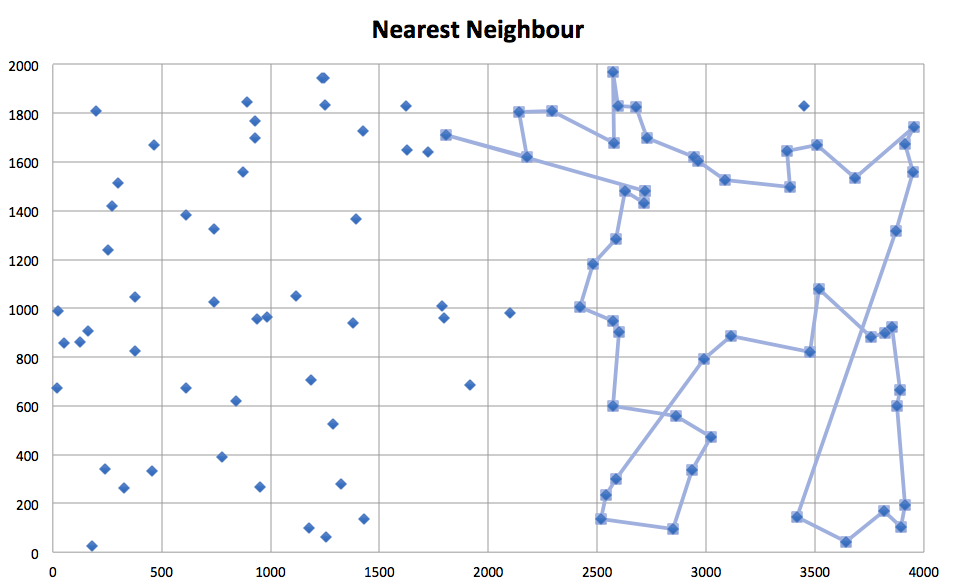
\includegraphics[angle=0,width = 1\textwidth, height=!]{images/NN.png}
\caption{Najlepsza trasa - Nearest Neighbour}
\label{Rys. NN}
\end{figure}

\section{Greedy Cycle}
\label{Greedy}
W algorytmie tym trasa jest budowana w taki sposób, aby zawsze tworzyła cykl Hamiltona. W każdej iteracji dodawany jest jeden najkrótszy łuk z pozostałych dostępnych.
\subsection{Implementacja w pseudokodzie}
\label{Greedy code}
\begin{lstlisting}[frame=single]
dla kazdego z zdefiniowanych punktow poczatkowych
	dodaj do sciezki punkt poczatkowy
	dla kazdego z punktow oprocz poczatkowego
		koszt = odleglosc pomiedzy tym punktem a poczatkowym
		jezeli koszt < dotychczasowy najmniejszy koszt
			dotychczasowy najmniejszy koszt = koszt
	koniec
	
	dodaj do sciezki punkt o najmniejszym koszcie (odleglosci)
	dodaj na koncu sciezki punkt poczatkowy
	
	dla pozostalych 48 krokow
		dla wszystkich par punktow w sciezce
			dla wszystkich nieodwiedzonych punktow
				koszt = odleglosc miedzy trojka punktow - odleglosc miedzy para punktow
				jezeli koszt < dotychczasowy najmniejszy koszt
					dotychczasowy najmniejszy koszt = koszt
			koniec
		koniec
		dodaj punkt powodujacy najmniejsza zmiane kosztu w odpowiednie miejsce w sciezce
	koniec	
koniec

\end{lstlisting}
\subsection{Wyniki}
\begin{table}[H]
\center
\caption{Greedy Cycle - wyniki}
\label{Greedy Cycle - wyniki}
\begin{tabular}{|p{1cm}|p{14cm}|}
\hline
min       & 11095                                                                                                                                                                                                 \\ \hline
mean      & 12653                                                                                                                                                                                                 \\ \hline
max       & 13393                                                                                                                                                                                                 \\ \hline
best path & 61, 34, 85, 26, 11, 19, 6, 8, 56, 86, 50, 24, 80, 60, 57, 66, 27, 92, 0, 7, 91, 74, 96, 18, 52, 15, 69, 21, 93, 87, 17, 23, 37, 83, 78, 89, 48, 5, 62, 46, 10, 16, 14, 31, 44, 90, 97, 22, 76, 59, 61 \\ \hline
\end{tabular}
\end{table}

\begin{figure} [H]
\centering
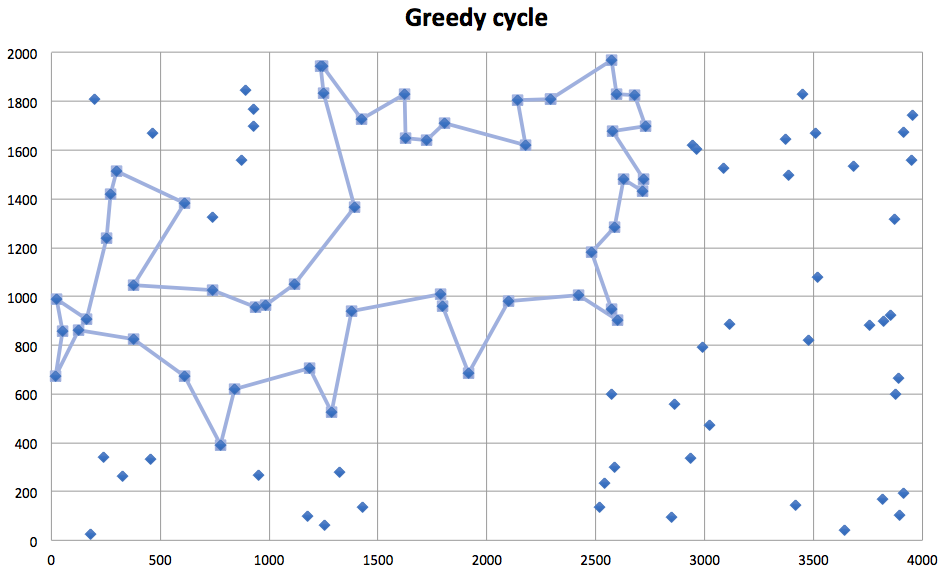
\includegraphics[angle=0,width = 1\textwidth, height=!]{images/GC.png}
\caption{Najlepsza trasa - Greedy Cycle}
\label{Rys. NN}
\end{figure}

\section{Nearest Neighbour Grasp}
Modyfikacja algorytmu Nearest Neighbour opisanego w punkcie \ref{Nearest} polegająca na tym, że w każdym kroku szukamy 3 najlepszych rozwiązań i z nich losujemy te, które będzie dodane do ścieżki.
\subsection{Implementacja w pseudokodzie}
Analogiczna do zawartej w podpunkcie \ref{Nearest code} z tą różnicą że zamiast szukać jednego punktu grafu znajdującego się najbliżej aktualnego punktu ścieżki należy znaleźć 3 najlepsze i wybrać losowy z nich.

\begin{lstlisting}[frame=single]
dla kazdego z zdefiniowanych punktow poczatkowych
	
	dodaj do sciezki punkt poczatkowy
			
	wykonaj 49 razy 
	
		dla kazdego punktow nie znajdujacych sie na sciezce
			koszt = odleglosc pomiedzy tym punktem a ostatnim dodanym do sciezki
			jezeli koszt < najwiekszy z listy 3 najmniejszych odleglosci
				dodaj koszt do listy 3 najmniejszych odleglosci zamiast najwiekszego z listy
		koniec
	
		dodaj do sciezki losowy z 3 punktow o najmniejszym koszcie (odleglosci)
		
	koniec	
	
	dodaj na koncu sciezki punkt poczatkowy
	
koniec

\end{lstlisting}

\subsection{Wyniki}

\begin{table}[H]
\center
\caption{Nearest Neighbour Grasp - wyniki}
\label{Nearest Neighbour Grasp- wyniki}
\begin{tabular}{|p{1cm}|p{14cm}|}
\hline
min       &  14103\\ \hline
mean      &  14146\\ \hline
max       &  21413\\ \hline
best path &  76
61
85
26
34
59
97
90
31
10
14
58
20
71
9 
48
5 
62
89
83
37
35
23
17
93
87
15
21
52
69
78
18
74
91
7 
55
30
41
79
88
0 
27
66
60
80
24
50
8 
6 
86
76 \\ \hline
\end{tabular}
\end{table}

\begin{figure} [H]
\centering
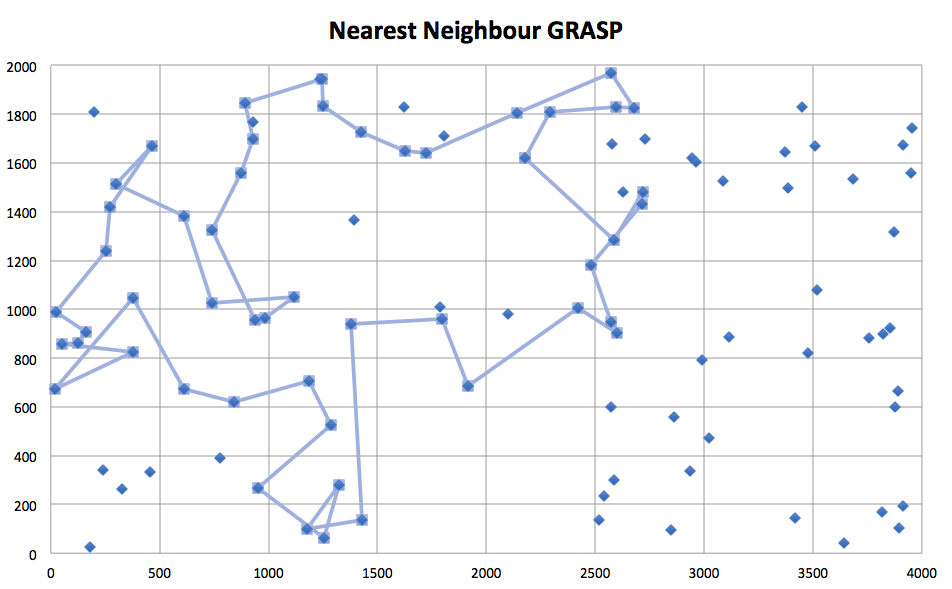
\includegraphics[angle=0,width = 1\textwidth, height=!]{images/NNG.png}
\caption{Najlepsza trasa - Nearest Neighbour Grasp}
\label{Rys. NNG}
\end{figure}
\section{Greedy Cycle Grasp}
Modyfikacja algorytmu Greedy Cycle opisanego w punkcie \ref{Greedy} polegająca na tym, że w każdym kroku szukamy 3 najlepszych rozwiązań i z nich losujemy te, które będzie dodane do ścieżki.
\subsection{Implementacja w pseudokodzie}
Analogiczna do zawartej w podpunkcie \ref{Greedy code} z tą różnicą że zamiast szukać jednej ścieżki która da najmniejsza różnice kosztów należy znaleźć 3 najlepsze trasy i wybrać losową z nich.

\begin{lstlisting}[frame=single]
dla kazdego z zdefiniowanych punktow poczatkowych
	dodaj do sciezki punkt poczatkowy
	dla kazdego z punktow oprocz poczatkowego
		koszt = odleglosc pomiedzy tym punktem a ostatnim dodanym do sciezki
			jezeli koszt < najwiekszy z listy 3 najmniejszych odleglosci
				dodaj koszt do listy 3 najmniejszych odleglosci zamiast najwiekszego z listy
		koniec
	
	dodaj do sciezki losowy z 3 punktow o najmniejszym koszcie (odleglosci)
	dodaj na koncu sciezki punkt poczatkowy
	
	dla pozostalych 48 krokow
		dla wszystkich par punktow w sciezce
			dla wszystkich nieodwiedzonych punktow
				koszt = odleglosc miedzy trojka punktow - odleglosc miedzy para punktow
				jezeli koszt < najwiekszy z listy 3 najmniejszych odleglosci
					dodaj koszt do listy 3 najmniejszych odleglosci zamiast najwiekszego z listy
			koniec
		koniec
		dodaj losowy punkt z 3 wybranych powodujacych najmniejsza zmiane kosztu w odpowiednie miejsce w sciezce
	koniec	
koniec

\end{lstlisting}
\subsection{Wyniki}

\begin{table}[H]
\center
\caption{Greedy Cycle Grasp - wyniki}
\label{Greedy Cycle Grasp- wyniki}
\begin{tabular}{|p{1cm}|p{14cm}|}
\hline
min       &  11095 \\ \hline
mean      &  13757 \\ \hline
max       &  13504 \\ \hline
best path &  61
34
85
26
11
19
6 
8 
56
86
50
24
80
60
57
66
27
92
0 
7 
91
74
96
18
52
15
69
21
93
87
17
23
37
83
78
89
48
5 
62
46
10
16
14
31
44
90
97
22
76
59
61\\ \hline
\end{tabular}
\end{table}

\begin{figure} [H]
\centering
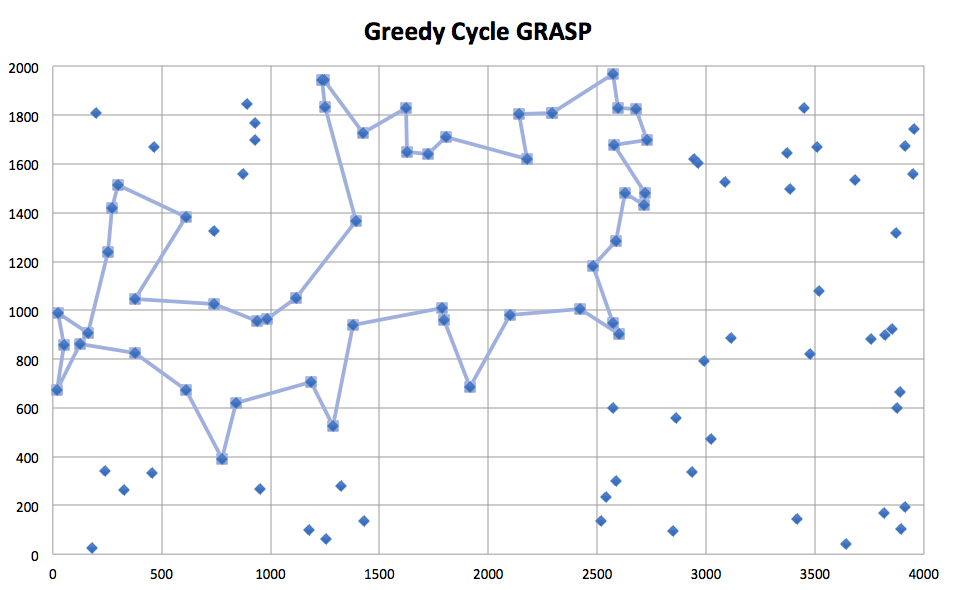
\includegraphics[angle=0,width = 1\textwidth, height=!]{images/GCG.png}
\caption{Najlepsza trasa - Greedy Cycle Grasp}
\label{Rys. GGC}
\end{figure}

\end{document}